\documentclass[../main.tex]{subfiles}
\begin{document}
\chapter{Multivariate Functions: Applications}
\section{Directional Derivatives and Gradient}
Consider $f(x, y)$ and a vector displacement $\d{\vec{s}}=(\d{x}, \d{y})$.
The infinitesimal change in $f$ along $\d{\vec{s}}$ is:
\begin{align*}
  \d{f} &= \pderiv{f}{x}\d{x} + \pderiv{f}{y}\d{y} \\
        &= (\d{x}, \d{y}) \cdot \left(\pderiv{f}{x}, \pderiv{f}{y}\right) \\
        &= \d{\vec{s}} \cdot \nabla f
\end{align*}
where $\nabla f$ is defined as follows.
\begin{definition}[Gradient of $f$]
  The  \textit{gradient of $f$} or grad $f$ is defined to be:
  \[
    \nabla f = \left(\pderiv{f}{x}, \pderiv{f}{y}\right)
  \]
\end{definition}
If we write $\d{\vec{s}} = \d{s}\uvec{s}$, where $\uvec{s}$ is a unit vector, then:
\[
  \d{f} = \d{s}\uvec{s} \cdot \nabla f
\]
\begin{definition}[Directional Derivative]
  The \textit{directional derivative} of $f$ in the direction of $\uvec{s}$ is:
  \[
    \deriv{f}{s} = \uvec{s} \cdot \nabla f
  \]
  where $\uvec{s}$ is a unit vector.
  This tells us the rate of change of $f(x, y)$ in the direction of $\uvec{s}$.
\end{definition}
\begin{center}
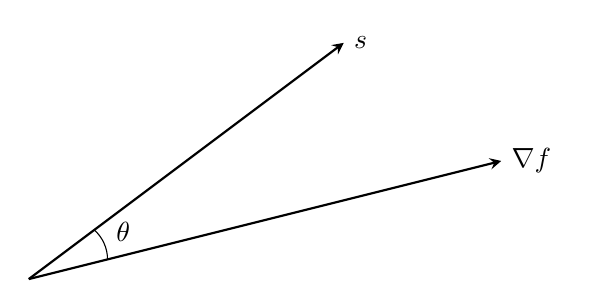
\begin{tikzpicture}[>=stealth, scale=1]
  \draw[->, thick] (0, 0) -- (4, 3) node[right] {$\uvec{s}$};
  \draw[->, thick] (0, 0) -- (6, 1.5) node[right] {$\nabla f$};

  \draw (1,0.25) arc[start angle=0, end angle=49, radius=0.5];

  \node at (1.2,0.6) {$\theta$};
\end{tikzpicture}
\end{center}
Using the definition of the scalar product, we see that:
\[
  \deriv{f}{s} = \uvec{s} \cdot \nabla f = \cos \theta |\nabla f|
\]
\begin{remark}[Note]
  As an alternative, we could have defined $\nabla f$ geometrically as the vector such that:
  \[
    \deriv{f}{s} = \uvec{s} \cdot \nabla f
  \]
  for all $\uvec{s}$.
\end{remark}
\subsection{Properties of the Gradient Vector}
\begin{enumerate}
  \item Direction of $\nabla f$ is that in which $f$ \textbf{increases} most rapidly as the directional derivative is greatest when $\uvec{s}$ is parallel to $\nabla f$
  \item The magnitude of $\nabla f$ is the max rate of change of $f$ at a particular point:
    \[
      |\nabla f| = \max_{\forall \theta}\left(\deriv{f}{s}\right)
    \]
  \item If $\uvec{s}$ is parallel to contours of $f$ (curves of constant $f$), then:
    \[
      \deriv{f}{s} = 0 = \uvec{s} \cdot \nabla f
    \]
    Therefore, $\nabla f$ is perpendicular to the contours of $f$.
\end{enumerate}
\section{Stationary Points}
There is always at least one direction where $\deriv{f}{s} = 0$, i.e. when $\uvec{s}$ is parallel to the contours of $f$.
So to define the notion of a stationary point, we require that $\deriv{f}{s} = 0$ in all directions, not just that $\deriv{f}{s} = 0$ for some $\uvec{s}$.
\begin{definition}[Stationary Point]
  A stationary point is a point where:
  \[
    \deriv{f}{s} = 0\ \forall \uvec{s}
  \]
\end{definition}
So at stationary points:
\[
  \vec{s} \cdot \nabla f = 0\ \forall \uvec{s} \implies \nabla f = \vec{0}
\]
\subsection{Types of Stationary Points}
\subsubsection{Local Maximum}
For a local maximum, $\nabla f$ points towards the maximum point.
Contours are usually locally elliptical around a maximum.
\begin{center}
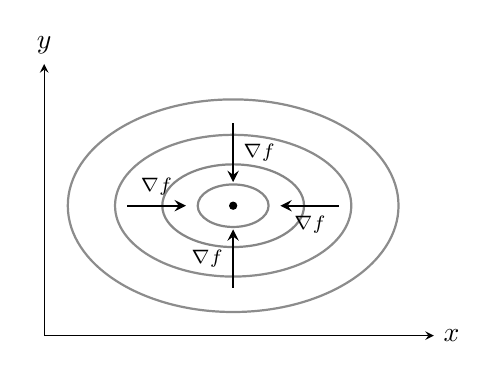
\begin{tikzpicture}[>=stealth, scale=1.5]
\draw[->] (0,0) -- (3.3,0) node[right] {$x$};
\draw[->] (0,0) -- (0,2.3) node[above] {$y$};

\def\cx{1.6}
\def\cy{1.1}

\draw[thick, gray!95] (\cx,\cy) ellipse (0.3 and 0.18);
\draw[thick, gray!95] (\cx,\cy) ellipse (0.6 and 0.35);
\draw[thick, gray!90] (\cx,\cy) ellipse (1.0 and 0.6);
\draw[thick, gray!90] (\cx,\cy) ellipse (1.4 and 0.9);

\fill (\cx,\cy) circle (1pt);

\draw[<-, thick] (\cx,\cy) + (0, -0.2) -- +(0, -0.7) node[midway, left] {$\scriptstyle\nabla f$};
\draw[<-, thick] (\cx,\cy) + (0, 0.2) -- +(0, 0.7) node[midway, right] {$\scriptstyle\nabla f$};
\draw[<-, thick] (\cx,\cy) + (0.4, 0) -- +(0.9, 0) node[midway, below] {$\scriptstyle\nabla f$};
\draw[<-, thick] (\cx,\cy) + (-0.4, 0) -- +(-0.9, 0) node[midway, above] {$\scriptstyle\nabla f$};
\end{tikzpicture}
\end{center}
\subsubsection{Local Minimum}
For a local minimum, $\nabla f$ points away from the minimum point.
Again, contours are usually locally elliptical.
\begin{center}
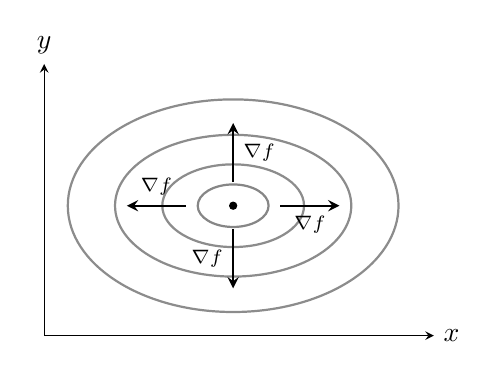
\begin{tikzpicture}[>=stealth, scale=1.5]
\draw[->] (0,0) -- (3.3,0) node[right] {$x$};
\draw[->] (0,0) -- (0,2.3) node[above] {$y$};

\def\cx{1.6}
\def\cy{1.1}

\draw[thick, gray!95] (\cx,\cy) ellipse (0.3 and 0.18);
\draw[thick, gray!90] (\cx,\cy) ellipse (0.6 and 0.35);
\draw[thick, gray!90] (\cx,\cy) ellipse (1.0 and 0.6);
\draw[thick, gray!90] (\cx,\cy) ellipse (1.4 and 0.9);

\fill (\cx,\cy) circle (1pt);

\draw[->, thick] (\cx,\cy) + (0, -0.2) -- +(0, -0.7) node[midway, left] {$\scriptstyle\nabla f$};
\draw[->, thick] (\cx,\cy) + (0, 0.2) -- +(0, 0.7) node[midway, right] {$\scriptstyle\nabla f$};
\draw[->, thick] (\cx,\cy) + (0.4, 0) -- +(0.9, 0) node[midway, below] {$\scriptstyle\nabla f$};
\draw[->, thick] (\cx,\cy) + (-0.4, 0) -- +(-0.9, 0) node[midway, above] {$\scriptstyle\nabla f$};
\end{tikzpicture}
\end{center}
\subsubsection{Saddle Point}
A saddle point is \textbf{not} a local extremum.
Generally speaking, in one direction it is a maximum and in another direction it is a minimum.
Contours always cross and only ever cross at a saddle points.
Around a saddle point, the contours are usually locally hyperbolic.
\begin{center}
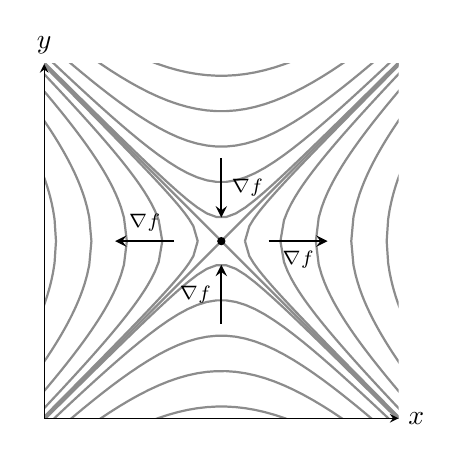
\begin{tikzpicture}[scale=1.5, >=stealth]
\def\cx{1.5}
\def\cy{1.5}
\begin{scope}
\clip (0, 0) rectangle (3, 3);
\foreach \b in {0.2, 0.5, 0.8, 1.1, 1.4}{
    \draw[thick, gray!90, domain=\cx+\b:\cx+2, samples=50] plot ({\x}, {\cy + sqrt((\x-\cx)^2 - \b^2)});
    \draw[thick, gray!90, domain=\cx+\b:\cx+2, samples=50] plot ({\x}, {\cy - sqrt((\x-\cx)^2 - \b^2)});
    \begin{scope}[xscale=-1, xshift=-3cm]
      \draw[thick, gray!90, domain=\cx+\b:\cx+2, samples=50] plot ({\x}, {\cy + sqrt((\x-\cx)^2 - \b^2)});
      \draw[thick, gray!90, domain=\cx+\b:\cx+2, samples=50] plot ({\x}, {\cy - sqrt((\x-\cx)^2 - \b^2)});
    \end{scope}
    \draw[thick, gray!90, domain=\cx-2:\cx+2, samples=50] plot ({\x}, {\cy + sqrt((\x-\cx)^2 + \b^2)});
    \draw[thick, gray!90, domain=\cx-2:\cx+2, samples=50] plot ({\x}, {\cy - sqrt((\x-\cx)^2 + \b^2)});
}
\draw[thick, gray!90] (\cx, \cy) + (-2, -2) -- +(2, 2);
\draw[thick, gray!90] (\cx, \cy) + (2, -2) -- +(-2, 2);
\end{scope}

\fill (\cx,\cy) circle (1pt);
\draw[<-, thick] (\cx,\cy) + (0, -0.2) -- +(0, -0.7) node[midway, left] {$\scriptstyle\nabla f$};
\draw[<-, thick] (\cx,\cy) + (0, 0.2) -- +(0, 0.7) node[midway, right] {$\scriptstyle\nabla f$};
\draw[->, thick] (\cx,\cy) + (0.4, 0) -- +(0.9, 0) node[midway, below] {$\scriptstyle\nabla f$};
\draw[->, thick] (\cx,\cy) + (-0.4, 0) -- +(-0.9, 0) node[midway, above] {$\scriptstyle\nabla f$};

\draw[->] (0,0) -- (3,0) node[right] {$x$};
\draw[->] (0,0) -- (0,3) node[above] {$y$};
\end{tikzpicture}
\end{center}
\section{Classification of Stationary Points}
How does $f$ change in the vicinity of a stationary point?
\subsection{Taylor Series for Multivariate Functions}
Consider how $f(x, y)$ varies along the line $\vec{x}(s) = \vec{x}_0 + s \uvec{s}$.
\begin{center}
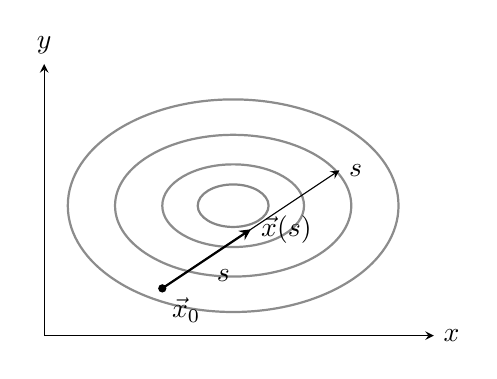
\begin{tikzpicture}[>=stealth, scale=1.5]
\draw[->] (0,0) -- (3.3,0) node[right] {$x$};
\draw[->] (0,0) -- (0,2.3) node[above] {$y$};

\def\cx{1.6}
\def\cy{1.1}

\draw[thick, gray!95] (\cx,\cy) ellipse (0.3 and 0.18);
\draw[thick, gray!90] (\cx,\cy) ellipse (0.6 and 0.35);
\draw[thick, gray!90] (\cx,\cy) ellipse (1.0 and 0.6);
\draw[thick, gray!90] (\cx,\cy) ellipse (1.4 and 0.9);

\coordinate (X) at (1, 0.4);
\fill (X) circle (1pt) node[below right] {$\vec{x}_0$};
\draw[->] (X) -- +(1.5, 1) node[right] {$\uvec{s}$};
\draw[->, thick] (X) -- +(0.75, 0.5) node[right] {$\vec{x}(s)$} node[midway, below right] {$s$};
\end{tikzpicture}
\end{center}
\end{center}
Along this line, $f(\vec{x}_0 + s \uvec{s}) = f(x(s), y(s))$ so $f$ is a function of $s$.
Therefore, we can use the usual Taylor series:
\begin{align*}
  f(\vec{x}_0 + s \uvec{s}) &= f(\vec{x}_0) + s \at{\deriv{f}{s}}{\vec{x}_0} + \frac{1}{2}s^2 \at{\deriv[2]{f}{s}}{\vec{x}_0} + \cdots \\
                            &= f(\vec{x}_0) + s \uvec{s} \cdot \at{\nabla f}{\vec{x}_0} + \frac{1}{2}s^2 \at{(\uvec{s} \cdot \nabla)(\uvec{s} \cdot \nabla f)}{\vec{x}_0} + \cdots
\end{align*}
Looking at the second term of the expansion, let $\delta\vec{x} = (x - x_0, y - y_0) = (\delta x, \delta y) = s \uvec{s}$.
We then have:
\[
  s \uvec{s} \cdot \nabla f = \delta \vec{x} \cdot \nabla f = \delta x \pderiv{f}{x} + \delta y \pderiv{f}{y}
\]
Looking at the third term of the expansion, let $\hat{s}_x$ and $\hat{s}_y$ be the components of $\uvec{s} =(\hat{s}_x, \hat{s}_y)$.
We then have:
\begin{align*}
  s^2(\uvec{s} \cdot \nabla)(\uvec{s} \cdot \nabla f) &= s^2\left(\hat{s}_x \pderiv{}{x} + \hat{s}_y \pderiv{}{y}\right)\left(\hat{s}_x \pderiv{f}{x} + \hat{s}_y \pderiv{f}{y}\right) \\
                                                      &= \left(\delta x \pderiv{}{x} + \delta y \pderiv{}{y}\right)\left(\delta x \pderiv{f}{x} + \delta y \pderiv{f}{y}\right) \\
                                                      &= (\delta x)^2 \pderiv[2]{f}{x} + (\delta x)(\delta y) \frac{\partial^2 f}{\partial x \partial y} + (\delta y)(\delta x)\frac{\partial^2 f}{\partial y \partial x} + (\delta y)^2 \pderiv[2]{f}{y} \\
                                                      &= (\delta x, \delta y)
                                                      \begin{pmatrix}
                                                      f_{x x} & f_{x y} \\
                                                      f_{y x} & f_{y y} \\
                                                      \end{pmatrix}
                                                      \begin{pmatrix}
                                                      \delta x \\
                                                      \delta y \\
                                                      \end{pmatrix}
\end{align*}
\begin{definition}[Hessian Matrix]
  The \textit{Hessian Matrix} is defined to be:
  \[
    H = \nabla \nabla f = \begin{pmatrix}
    f_{x x} & f_{x y} \\
    f_{y x} & f_{y y} \\
    \end{pmatrix}
  \]
  This is symmetric as $f_{x y} = f_{y x}$.
\end{definition}
The multivariate Taylor series is then:
\begin{align*}
  f(x_0 + \delta x, y_0 + \delta y) &= f(x_0, y_0) + \at{\left[\delta x \pderiv{f}{x} + \delta y \pderiv{f}{y}\right]}{(x_0, y_0)} \\ &\quad+\frac{1}{2}\at{\left[(\delta x)^2 \pderiv[2]{f}{x} + 2\delta x\delta y \frac{\partial^2 f}{\partial x \partial y} + (\delta y)^2 \pderiv[2]{f}{y}\right]}{(x_0, y_0)} + \cdots
\end{align*}
This can be written in a coordinate independent form as:
\begin{align*}
  f(\vec{x}_0 + \delta \vec{x}) &= f(\vec{x}_0) + \delta \vec{x} \cdot \at{(\nabla f)}{\vec{x}_0} + \frac{1}{2} (\delta \vec{x})^{\trans} \at{H}{\vec{x}_0} \delta \vec{x} + \cdots \\
                                & =f(\vec{x}_0) + \delta \vec{x} \cdot \at{(\nabla f)}{\vec{x}_0} + \frac{1}{2} (\delta \vec{x})^{\trans} \at{(\nabla \nabla f)}{\vec{x}_0} \delta \vec{x} + \cdots
\end{align*}
\end{document}
